
\section{Calibração Intrínseca}

Para realização da calibração intrínseca da câmera, foram tomadas duas capturas de um objeto de calibração, sendo essa, uma caixa conhecida com 275 mm de altura, 87 mm de largura e 150 mm de profundidade. A \autoref{fig:i7_L} apresenta a vista esquerda da caixa, enquanto na \autoref{fig:i7_R} foi capturada a vista direita do objeto. Ambas as imagens foram capturadas pela mesma câmera, tendo tamanho de $640 \times 480$ pixels.

\begin{figure}[H]
	\centering
	\begin{subfigure}[H]{0.49\textwidth}
		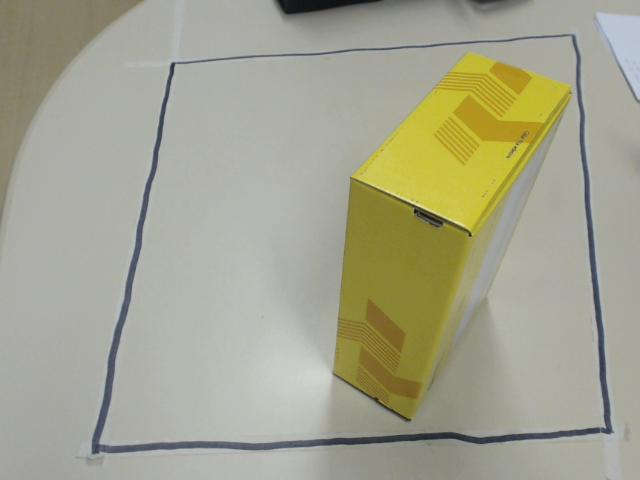
\includegraphics[width = \textwidth]{../../data/i7_L.jpg}
		\caption{Vista esquerda.}
		\label{fig:i7_L}
	\end{subfigure}
	\begin{subfigure}[H]{0.49\textwidth}
		\centering
		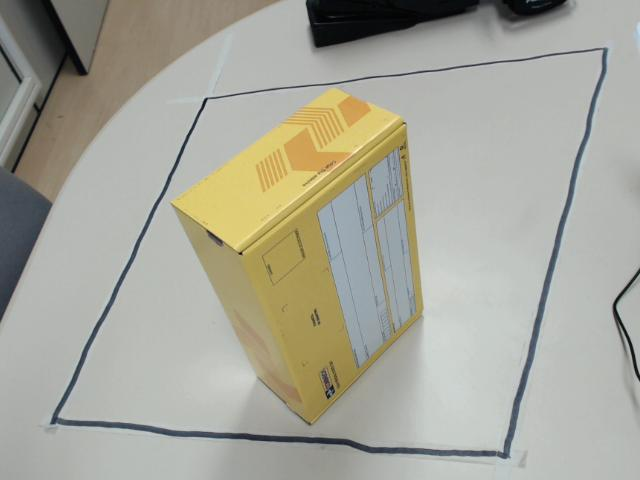
\includegraphics[width = \textwidth]{../../data/i7_R.jpg}
		\caption{Vista direita.}
		\label{fig:i7_R}
	\end{subfigure}
	\caption{Imagens de calibração.}
\end{figure}

\subsection{Obtenção de pontos}

A definição dos pontos do sólido de calibração que serão utilizados para a calibração é crucial, tendo sido realizado de forma manual por meio do \textit{software} de edição de imagens Adobe Photoshop. Os pontos são enumerados para corresponder ao vetor de pontos conhecidos utilizados na função de calibração, sendo o sistema global de coordenadas tendo origem no ponto $\mathit{1}$ e os eixos definidos nas direções:

\begin{align}
	\text{Eixo } z \equiv \overrightarrow{\mathit{1} \to \mathit{6}} \\
	\text{Eixo } x \equiv \overrightarrow{\mathit{1} \to \mathit{2}} \\
	\text{Eixo } y \equiv \overrightarrow{\mathit{1} \to \mathit{7}}
\end{align}

O ponto oculto foi estimado por meio da projeção das arestas ocultas do sólido, por meio do paralelismo com as arestas visíveis, onde o ponto de interseção foi aproximado como o oitavo vértice do paralelepípedo.

\begin{figure}[H]
	\centering
	\begin{subfigure}[H]{0.49\textwidth}
		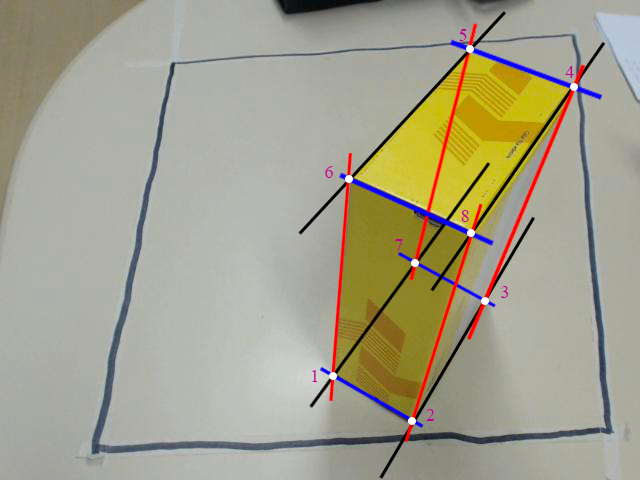
\includegraphics[width = \textwidth]{../../data/i7_L_axis.png}
		\caption{Vista esquerda.}
		\label{fig:i7_L_axis}
	\end{subfigure}
	\begin{subfigure}[H]{0.49\textwidth}
		\centering
		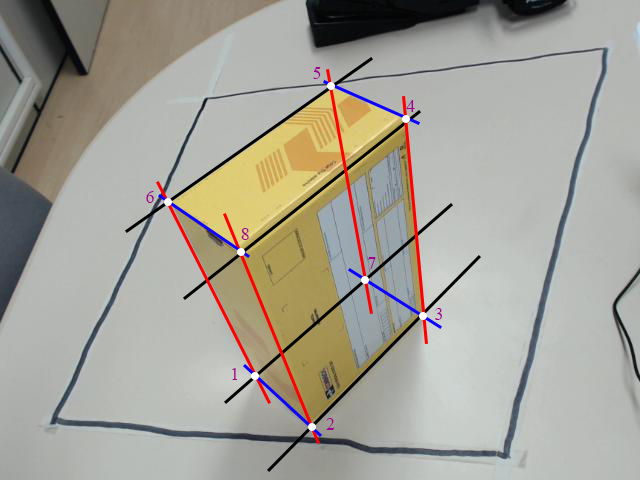
\includegraphics[width = \textwidth]{../../data/i7_R_axis.png}
		\caption{Vista direita.}
		\label{fig:i7_R_axis}
	\end{subfigure}
	\caption{Imagens de calibração com pontos conhecidos do mundo destacados.}
\end{figure}

Os pontos foram amostrados manualmente da imagem com os eixos, utilizando a função \texttt{getpts} do \textsc{Matlab}, resultando em dois vetores, com as coordenadas $x$ e $y$ de cada ponto. Dado as coordenadas, os mesmos foram utilizados para montar a matriz de pontos de calibração, com o mesmo padrão mostrado em \eqref{eq:mpoints}, sendo \texttt{ceil()} a função de truncamento para obtenção da coordenada de imagem do ponto, sendo obtida uma matriz de pontos para cada imagem. A notação com subscrito $L$ será adotada para as equações relativas à imagem da vista esquerda, e o subscrito $R$ para a vista direita.

\begin{equation}\label{eq:mpoints}
	\+{\hat{p}} = \begin{bmatrix}
		\texttt{ceil(}\vec{x}\texttt{)}_{[1 \times 8]} \\
		\texttt{ceil(}\vec{y}\texttt{)}_{[1 \times 8]} \\
		\mathbf{1}
	\end{bmatrix}_{[3 \times 8]}
\end{equation}

Dados os pontos em coordenadas de mundo do sólido de calibração, em metros, dado por \eqref{eq:B}, obteve-se as matrizes com os pontos relativos em coordenadas de imagem para a imagem da vista esquerda, \eqref{eq:pL}, e para a vista direita, \eqref{eq:pR}.

\begin{equation} \label{eq:B}
	\+B = \begin{bmatrix}
			0 & 0.087 & 0.087 & 0.087 & 0     & 0     & 0     & 0.087 \\
			0 & 0     & 0.150 & 0.150 & 0.150 & 0     & 0.150 & 0     \\
			0 & 0     & 0     & 0.275 & 0.275 & 0.275 & 0     & 0.275
	\end{bmatrix}
\end{equation}

\begin{equation} \label{eq:pL}
	\+{\hat{p}}_L = \begin{bmatrix}
		334 & 412 & 486 & 575 & 470 & 350 & 416 & 472 \\
		377 & 423 & 302 & 89  & 50  & 180 & 265 & 235 \\
		1   & 1   & 1   & 1   & 1   & 1   & 1   & 1  
	\end{bmatrix}
\end{equation}

\begin{equation} \label{eq:pR}
	\+{\hat{p}}_R = \begin{bmatrix}
		256 & 312 & 424 & 407 & 331 & 169 & 366 & 242 \\
		378 & 428 & 317 & 121 & 86  & 203 & 282 & 253 \\
		1   & 1   & 1   & 1   & 1   & 1   & 1   & 1 
	\end{bmatrix}
\end{equation}

Com a aplicação da função de calibração intrínseca \texttt{RTAa()}, obtém-se a matriz de parâmetros intrínsecos aproximada ($\mathbf{\hat{A}}$), a matriz de rotação aproximada ($\mathbf{\hat{R}}$) e o vetor de translação aproximado ($\mathbf{\hat{t}}$), sendo os dois últimos em relação à câmera e o sistema de coordenadas do mundo, ou seja, serão diferentes para cada uma das imagens.

Para a vista esquerda (\autoref{fig:i7_L_axis}), foram obtidas as seguintes matrizes:

\begin{gather}\label{eq:ve}
\+{\hat{A}}_L = \begin{bmatrix}
	630.8066 & 0        & 426.9824 \\
	0        & 634.6096 & 216.9257 \\
	0        & 0        & 1  
\end{bmatrix}; \\ \ \+{\hat{R}}_L = \begin{bmatrix}
	0.8682  & 0.4806  & 0.1239  \\
	0.4416  & -0.6343 & -0.6345 \\
	-0.2263 & 0.6055  & -0.7630
\end{bmatrix}; \ \+{\hat{t}}_L = \begin{bmatrix}
	0.1366 \\
	-0.2138 \\
	0.5406
\end{bmatrix};  \label{eq:rtL}
\end{gather}

Para a vista direita (\autoref{fig:i7_R_axis}), foram obtidas as seguintes matrizes:

\begin{gather}\label{eq:vd}
	\+{\hat{A}}_R = \begin{bmatrix}
	648.0318 & 0        & 330.0854 \\
	0        & 607.4200 & 200.7036 \\
	0        & 0        & 1
	\end{bmatrix}; \\ \ \+{\hat{R}}_R = \begin{bmatrix}
	0.6871  & 0.7023  & -0.1861 \\
	0.4168  & -0.5909 & -0.6908 \\
	-0.5951 & 0.3971  & -0.6987
	\end{bmatrix}; \ \+{\hat{t}}_R = \begin{bmatrix}
	0.3318 \\
	-0.0902 \\
	0.5437
	\end{bmatrix}; \label{eq:rtR}
\end{gather}

Por fim, para uma melhor realização da matriz de parâmetros intrínsecos aproximada, tira-se a média das duas aproximações obtidas, tendo então:

\begin{equation}\label{eq:amed}
	\+{\hat{A}} = \begin{bmatrix}
		639.4192 & 0        & 378.5339 \\
		0        & 621.0148 & 208.8146 \\
		0        & 0        & 1 		
	\end{bmatrix}
\end{equation}


\clearpage
\section{Transformação entre às câmeras}

A matriz de rotação e o vetor de translação entre a câmera e o sistema de coordenadas do mundo podem ser representadas na forma de transformações homogêneas, que compactam a informação de rotação e translação, sendo construída com base em \eqref{eq:th}.

\begin{equation}
	\+T = \begin{bmatrix}
	&	\+R_{[3\times 3]} & & \+{t}_{[3\times 1]} \\
		0 & 0 & 0 & 1
	\end{bmatrix}_{[4\times 4]}
	\label{eq:th}
\end{equation}

Para a transformação entre dois \textit{frames} $\{2\}$ e $\{1\}$ quaisquer, tem-se \eqref{eq:th21}.

\begin{equation}
\+T_{2/1} = \begin{bmatrix}
	& \+R_{2/1} & & \+{t}_{2/1} \\
	0 & 0 & 0 & 1
\end{bmatrix}
\label{eq:th21}
\end{equation}

De acordo com a propriedade algébrica das transformações homogêneas, a transformação do \textit{frame} $\{0\}$ para o $\{2\}$ pode ser decomposta no produto da transformação do \textit{frame} $\{0\}$ para o $\{1\}$, e do   \textit{frame} $\{1\}$ para o $\{2\}$.

\begin{equation}
	\+T_{0/2} = \+T_{2/1} \+T_{1/0} \therefore \+T_{2/1} = \+T_{0/2} \+T_{1/0} = \+T_{0/2} \+T^{-1}_{0/1}
\end{equation}

Dessa forma, uma vez que se conhece a transformação da câmera na vista esquerda para o sistema do mundo, e a transformação da câmera na vista direita para o sistema do mundo, a tranformação entre as duas câmeras pode ser encontrada da forma \eqref{eq:tfLR}.

\begin{equation}
	\+{\hat{T}}_{R/L} = \+{\hat{T}}_{R/0}\+{\hat{T}}_{0/L} =  \+{\hat{T}}_{R/0}\+{\hat{T}}_{L/0}^{-1}
	\label{eq:tfLR}
\end{equation}

Com base em \eqref{eq:rtL}, pode-se escrever a transformação homogênea da câmera $L$ para o sistema de coordenadas do mundo como \eqref{eq:TL}.

\begin{equation}\label{eq:TL}
	\+{\hat{T}}_{L/0} = \begin{bmatrix}
		& \+{\hat{R}}_L & & \+{\hat{t}}_L\\
		0 & 0 & 0 & 1
	\end{bmatrix} = \begin{bmatrix}
	0.8682  & 0.4806  & 0.1239  & 0.1366  \\
	0.4416  & -0.6343 & -0.6345 & -0.2138 \\
	-0.2263 & 0.6055  & -0.7630 & 0.5406  \\
	0       & 0       & 0       & 1  
\end{bmatrix}
\end{equation}  

E por meio da \eqref{eq:rtR}, pode-se escrever a transformação homogênea da câmera $R$ para o sistema de coordenadas do mundo como \eqref{eq:TR}.

\begin{equation}\label{eq:TR}
 	\+{\hat{T}}_{R/0} = \begin{bmatrix}
 		& \+{\hat{R}}_R & & \+{\hat{t}}_R\\
 		0 & 0 & 0 & 1
 	\end{bmatrix} = \begin{bmatrix}
 	0.6871  & 0.7023  & -0.1861 & 0.3318  \\
 	0.4168  & -0.5909 & -0.6908 & -0.0902 \\
 	-0.5951 & 0.3971  & -0.6987 & 0.5437  \\
 	0       & 0       & 0       & 1
 \end{bmatrix}
\end{equation} 


Com isso, de acordo com \eqref{eq:tfLR}, têm-se que, a transformação do referencial da câmera da esquerda para a câmera da direta é expressa por \eqref{eq:tfL2R} e a transformação da câmera da direta para a câmera da esquerda é dada por \eqref{eq:tfR2L}.

\begin{equation}\label{eq:tfL2R}
	\+{\hat{T}}_{L/R} = \begin{bmatrix}
		0.9153  & 0.2589 & -0.3085 & 0.2233  \\
		-0.2945 & 0.9527 & -0.0743 & 0.0173  \\
		0.2747  & 0.1589 & 0.9483  & -0.0566 \\
		0       & 0      & 0       & 1   
	\end{bmatrix}
\end{equation}

\begin{equation}\label{eq:tfR2L}
	\+{\hat{T}}_{R/L} = \begin{bmatrix}
		0.9153  & -0.2945 & 0.2747 & -0.1838 \\
		0.2589  & 0.9527  & 0.1589 & -0.0653 \\
		-0.3085 & -0.0743 & 0.9483 & 0.1239  \\
		0       & 0       & 0      & 1
	\end{bmatrix}
\end{equation}

Explicitando as matrizes de rotação e vetores de translação entre às cameras:

\begin{gather}
	\+{\hat{R}}_{L/R} = \begin{bmatrix}
		0.9153  & 0.2589 & -0.3085 \\
		-0.2945 & 0.9527 & -0.0743 \\
		0.2747  & 0.1589 & 0.9483 
	\end{bmatrix}; \ \+{\hat{t}}_{L/R} = \begin{bmatrix}
		0.2233 \\
		0.0173 \\
		-0.0566
	\end{bmatrix};
\end{gather}

\begin{gather}
\+{\hat{R}}_{R/L} = \begin{bmatrix}
	0.9153  & -0.2945 & 0.2747 \\
	0.2589  & 0.9527  & 0.1589 \\
	-0.3085 & -0.0743 & 0.9483
\end{bmatrix}; \ \+{\hat{t}}_{R/L} = \begin{bmatrix}
	-0.1838 \\
	-0.0653 \\
	0.1239
\end{bmatrix}; 
\end{gather}

\clearpage
\section{Conclusão}